\chapter{Stochastic Tractography}
\begin{figure} \label{fig:stflow}
	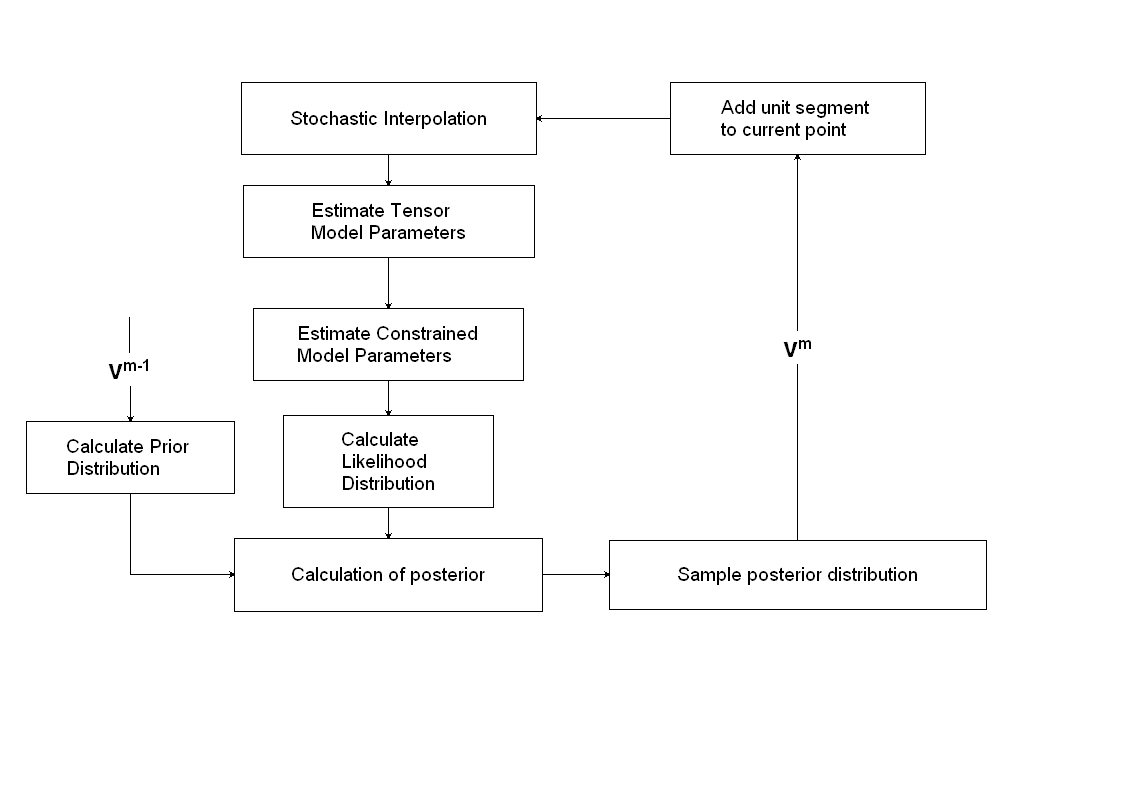
\includegraphics[width=\linewidth]{stflow}
	\caption{A flow chart demonstrating key steps in the stochastic tractgraphy algorithm}
\end{figure}
The Stochastic Tractography System implemented in this research implements Friman's \cite{frimanTMI06} approach to Stochastic Tractography with some modifications to the stopping criteria.

Friman's approach is a bayesian based inference algorithm similar to Behren's but with some optimizations to Behrens's approach \cite{frimanTMI06}.  In contrast with Behrens's two-compartment observation model, the model used by Friman is derived from the thoroughly studied tensor model of diffusion.  Friman uses a contrained diffusion observation model.  In this model, the two smallest eigenvectors of diffusion tensor are equal, constraining the shape of the diffusion tensor to be more linear if anisotropy exists.  The constrained model essentially rules out the possiblity of planar anistropic diffusion distributions.  Deviations from linearly anisotropic diffusion distributions are captured as uncertainty in the fiber orientation.  The advantage of using the constrained model is that it is relately easy to estimate the parameters for the model.  The parameters for the constrained model are obtained easily after the tensor model has been fit to the diffusion data.  Since the parameters for the tensor model are easily optained through many computationally efficient ways, the contrained model's parameters are likewise easy to obtain.  The constrained model is able can be fit to every voxel within a matter of seconds whereas Behrens model takes a couple of hours \cite{frimanTMI06}.  Additionally Friman avoids using MCMC techniques by assuming that parameters other than the principle diffusion direction take on their ML estimates with certainty within each voxel.  Friman demonstrates that eliminating this source of uncertainty has little effect on the resulting posterior fiber orientation distribution.

In Friman's paper on stochastic tractography, the tracking was terminated when an encountered voxel was too isotropic.  However, since the stochastic tractography algorithm takes into account this uncertainty with an increase in the spatial variance of sampled fibers, this termination criteria seems arbitrary and contradictory with the goals of stochastic tractography, which is to enable sampling of tracts in regions of uncertainty.  Thus this termination criteria has been replaced with a criteria which terminates tractography based on posterior probability that a fiber tract exists within the current voxel.  The posterior probability that a fiber tract exists in a given voxel can be obtained by performing a soft segmentation of white matter on an anatomical image coregistered with the DWI data.  Alternatively, the soft segmentation can also be performed on the B0 image of the DWI data set, thus eliminating the need for additional data.  Although this may seem equivalent to using fractional anisotropy since white matter generally has higher anisotropy than grey matter, it does not exclude isotropic regions of white matter which have crossing fibers.  Theoretically, this should enable the algorithm to detect more tracts than it would have otherwise under the anisotropy termination criteria.
%talk through key portions of the math
%present a block diagram of the algorithm




%need to add in a bit about how they are different in the way they sample the PDF

%talk about how it differs from other algorithms
%talk about using incorporating the posterior probability of white matter
%talk about why we choose to segment the gray/white matter using b0 image instead of using diffusion information
